\providecommand\boxheight[1]{#1cm} % a box's height in cm, unless the exam redefines it
\titledquestion{Centrality} Consider the following network
\begin{equation*}
    G = \begin{pmatrix}
        1 & 1 & 1 \\
        1 & 1 & 1 \\
        1 & 1 & 1 \\
    \end{pmatrix}.
    \end{equation*}
Let $\beta_i = 1$ be the exogenous importance of each node.

\begin{parts}
    \part[3] Draw the network.
    \begin{solutionorbox}[\boxheight{10}]
        
        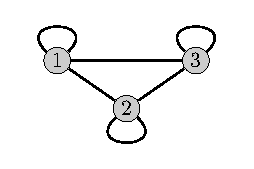
\includegraphics{centrality/centrality-simple_complete}
    \end{solutionorbox}
    \ifdefined\exambreak\exambreak\fi % an exam may start this part on a new page (its box does not fit under the part before)
    \part[7] Compute the Katz-Bonacich centrality for each node of the network for a suitable range of $\alpha$.

    \begin{solutionorbox}[\boxheight{20}]
        \begin{enumerate}
            \item   Note that 
        \begin{equation*}
            G = 3 \underbrace{\begin{pmatrix}
                \frac{1}{3} & \frac{1}{3} & \frac{1}{3} \\
                \frac{1}{3} & \frac{1}{3} & \frac{1}{3} \\
                \frac{1}{3} & \frac{1}{3} & \frac{1}{3} \\
            \end{pmatrix}}_{=: \tilde G},
        \end{equation*}
        where $\tilde G$ is of the form \begin{equation*}
            \begin{pmatrix}
                \bm \pi^T \\ \bm \pi^T \\ \bm \pi^T
            \end{pmatrix}.
        \end{equation*}
        where $\bm \pi^T \in \mathbb{R}^{1 \times n}$ is a stochastic row vector. 
        \item Thus, by the stationary-matrix theorem, $G^i = (3 \tilde G)^i = 3^i \tilde G^i = 3^i \tilde G$ for all $i \geq 1$.
        \item The Katz-Bonacich centrality is given by \begin{equation*}
            \tilde{\bm c}^{\text{KB}} = \Bigl(\sum_{i=1}^\infty \alpha^i G^i\Bigr)^T \bm \beta
        \end{equation*}
        \item The infinite sum is
        \begin{equation*}
            \sum_{i=1}^\infty \alpha^i \underbrace{G^i}_{3^i \tilde G} = \tilde G \sum_{i = 1}^\infty (3\alpha)^i = \frac{3\alpha}{1-3\alpha} \tilde G
        \end{equation*}
        if and only if $3\alpha < 1 \iff \alpha < \frac{1}{3}$. ($\alpha$ cannot be negative.) Otherwise the sum diverges to $+\infty$.
        \item We continue under the assumption that $\alpha \in (0, \frac{1}{3}$)
        \item So, 
        \begin{equation*}
            \tilde{\bm c}^{\text{KB}} = \frac{3\alpha}{1-3\alpha} \tilde G^T \bm \beta = \frac{3\alpha}{1-3\alpha} 
        \begin{pmatrix}
            \frac{1}{3} & \frac{1}{3} & \frac{1}{3} \\
            \frac{1}{3} & \frac{1}{3} & \frac{1}{3} \\
            \frac{1}{3} & \frac{1}{3} & \frac{1}{3} \\
        \end{pmatrix} \begin{pmatrix}
            1 \\ 1 \\1 
        \end{pmatrix} = \frac{3\alpha}{1-3\alpha} \begin{pmatrix}
            1 \\ 1 \\1 
        \end{pmatrix}
    \end{equation*}
       \item So $\tilde{c}^{\text{KB}}_i =  \frac{3\alpha}{1 - 3\alpha}$ for each node $i$, as long as $\alpha \in (0, \frac{1}{3}$).
    \end{enumerate}
    \end{solutionorbox}
\end{parts}